\documentclass[a4paper, 12pt]{scrartcl}
\usepackage{scrpage2}
\usepackage[left=2.5cm,right=2.5cm, top=3cm, bottom=4cm]{geometry}
\usepackage[utf8]{inputenc}
\usepackage[ngerman]{babel}
\usepackage[T1]{fontenc}
\usepackage{amsmath}
\usepackage{amssymb}
\usepackage{amsfonts}

\usepackage{graphicx}

\usepackage{float}
\usepackage{adjustbox}
\usepackage{hyperref}
\usepackage{textcomp}
\usepackage{multirow}
\usepackage{array}

%\usepackage{enumerate}
\usepackage[shortlabels]{enumitem}

%Zeichnungen
\usepackage{tikz}
\usepackage[european]{circuitikz}

% Einrücken verhindern
\setlength{\parindent}{0em} 


\begin{document}

\begin{titlepage}
	\centering
	{\Huge\bfseries Versuchsprotokoll\par}
	\vspace{2cm}
	{\scshape\LARGE Elektrizitätslehre \par}
	\vspace{1cm}
	{\Large Gedämpfter LCR-Schwingkreis und \\ Gekoppelte LC-Schwingkreise\par}
	\vfill
	{\large\itshape Simon Schwarz und Marius Ising\par}

	\vfill
\end{titlepage}

\tableofcontents
\newpage


\section{Gedämpfter LCR-Schwingkreis}


\subsection{Versuchsbeschreibung}

In einer Serienschaltung aus Spule $L$, Kondensator $C$ und Ohmschem Widerstand $R$ (vgl. Abb. \ref{abb:schaltLCR}) wird der Kondensator zunächst aufgeladen und anschließend die Spannungsquelle mit einem Taster überbrückt, sodass der Kondensator sich über den Widerstand entladen kann. Dabei entlädt sich der Kondensator nicht sofort, sondern er schwingt sich bei der Spannung $U=0$ ein. Dieser Einschwingvorgang hängt wesentlich von der Dämpfung der Schwingung durch die Ohmschen Widerstände der Schaltung ab.

\begin{figure}[H]
\centering
\begin{tikzpicture}
\draw (2,0) node[ocirc]{} -- (2,1) to [C, a=$C$] (2,3) to [R, a=$R$] (4,3)  to [cute inductor, a=$L$] (6,3) to[rmeterwa, t=$I$] (6,1) -- (6,0) node[ocirc]{};
\draw (2,1) to [push button] (6,1);
\draw (2,1.2) -- (1,1.2) to [rmeterwa, t=$U_C$] (1,2.8) -- (2,2.8);
\end{tikzpicture}
\caption{Schaltbild des LCR-Schwingkreises}
\label{abb:schaltLCR}
\end{figure}

Nach der Kirchhoffschen Maschenregel gilt für die Schaltung bei gedrücktem Taster
$$0 = U_C + U_R + U_L = \frac QC + RI + L \frac{dI}{dt}$$
Mit $I = \frac{dQ}{dt}$ erhält man folgende Differentialgleichung
$$\frac{d^2Q}{dt^2} + \frac{R}{L} \frac{dQ}{dt} + \frac{1}{LC}Q = 0$$
Dies ist die DGL einer gedämpften harmonischen Schwingung. Dabei bezeichnet $\delta = \frac{R}{2L}$ die Dämpfungskonstante und $\omega_0 = \frac{1}{\sqrt{LC}}$ die Schwingungsfrequenz der ungedämpften Schwingung. 
Für die Lösung der DGL unterscheiden wir drei Fälle. In allen Fällen gelten die gleichen Anfangsbedingungen
$$Q(0) = CU_0 \hspace{0.5cm} \text{ und } \hspace{0.5cm} I(0) = 0.$$

\textbf{Schwingfall ($\delta < \omega_0$)} \\
Hier ist eine echte Schwingung zu beobachten. Es gilt
$$Q(t) = e^{-\delta t}( A\cos(\omega t) + B\sin(\omega t)).$$
Aus den Anfangsbedingungen erhält man $A = CU_0$ und $B = A \frac{\delta}{\omega}$. Für den Strom gilt wegen $I = \frac{dQ}{dt}$
\begin{equation}\label{eq:i_lsg}
I(t) = -CU_0 e^{-\delta t} \left( \omega + \frac{\delta^2}{\omega}\right)\sin(\omega t)\text{.}
\end{equation}

\textbf{Kriechfall ($\delta > \omega_0$)} \\ 
In diesem Fall ist die Dämpfung so stark, dass der Kondensator seine Spannung nur sehr langsam verliert. Zudem findet keine Schwingung statt.
$$Q(t) = Ae^{\left( -\delta + \sqrt{\delta^2-\omega_0^2} \right)t} + Be^{\left(-\delta - \sqrt{\delta^2-\omega_0^2} \right)t}$$
Aus den Anfangsbedingungen ergibt sich
$$A = CU_0 \frac{\delta +\sqrt{\delta^2-\omega_0^2}}{2\sqrt{\delta^2-\omega_0^2}} \hspace{0.5cm} \text{ und } \hspace{0.5cm}
B = CU_0 \frac{-\delta+\sqrt{\delta^2-\omega_0^2}}{2\sqrt{\delta^2-\omega_0^2}}$$

\textbf{Aperiodischer Grenzfall ($\delta = \omega_0$)} \\
Der Kondensator wird innerhalb der kürzesten Zeit entladen. Die Lösung hat die Form
$$Q(t) = e^{-\delta t}(A + Bt)$$
mit $A = CU_0$ und $B=\delta A$.


\subsection{Versuchsaufbau}

\begin{figure}[H]
\centering
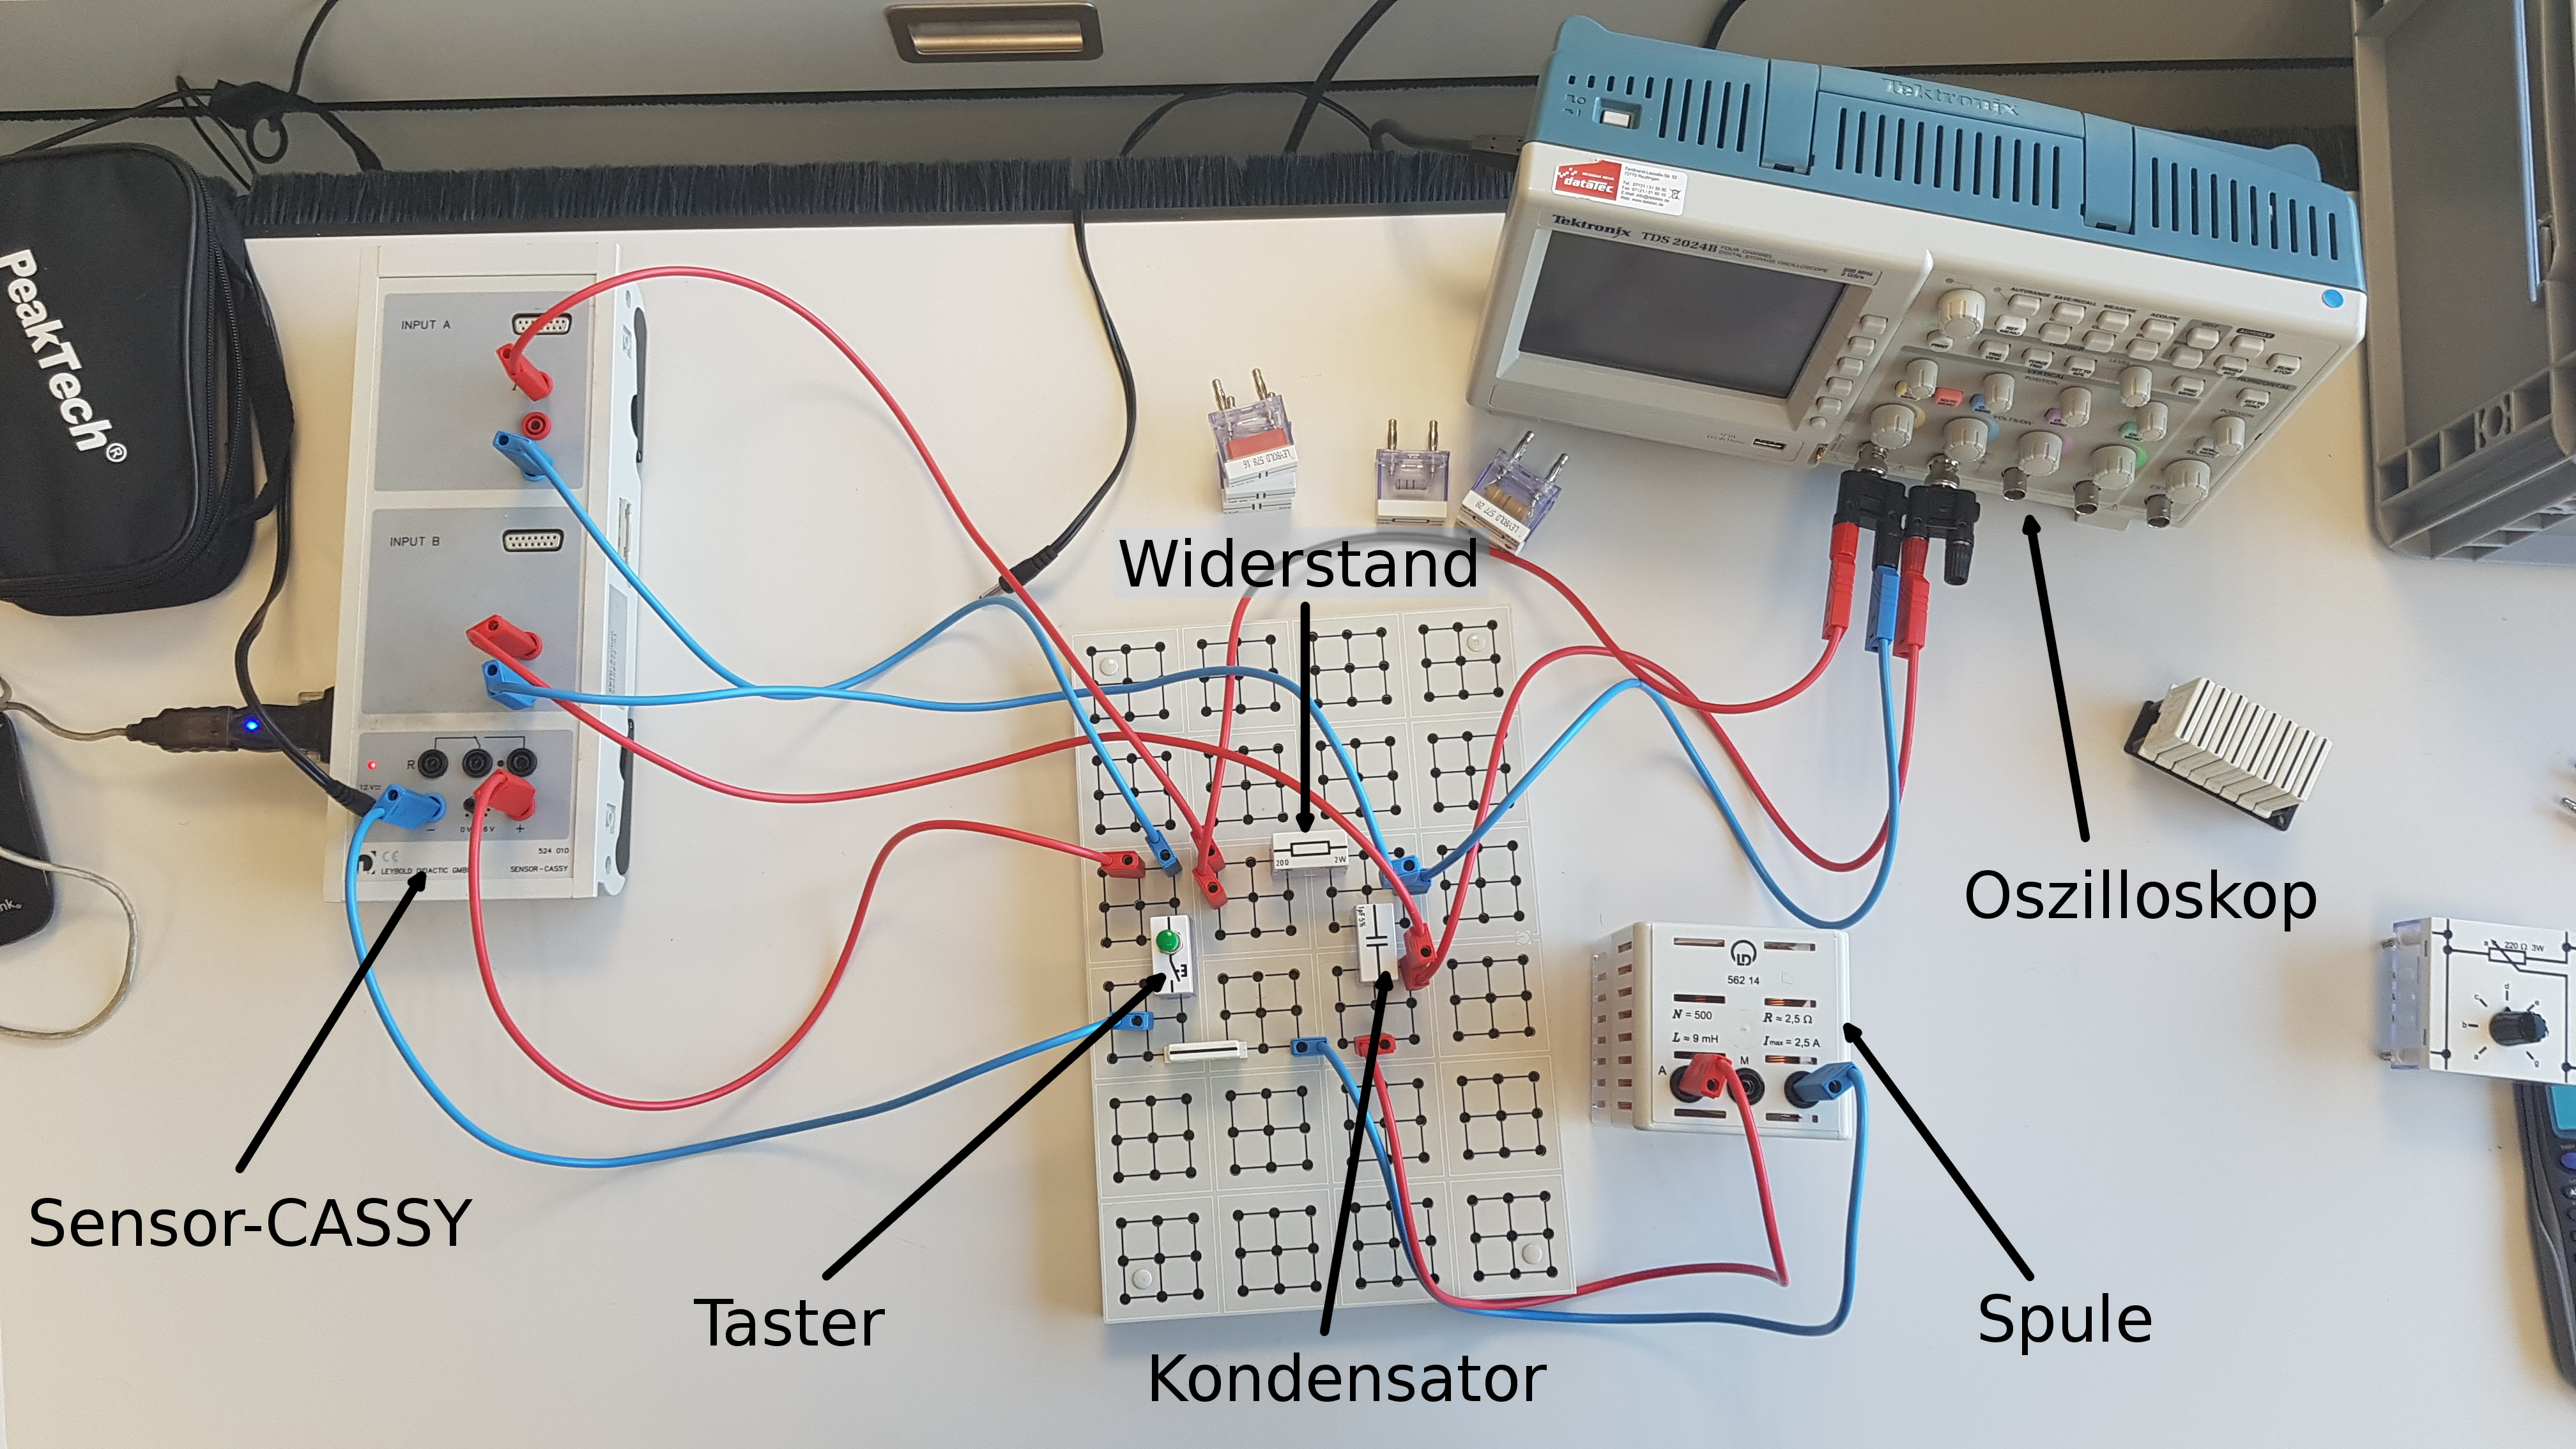
\includegraphics[width=\textwidth]{bilder/LCR_aufbau_beschriftet.jpg}
\caption{Versuchsaufbau LCR-Schwingkreis}
\label{abb:aufbau_lcr}
\end{figure}
Das Schaltbild aus Abbildung \ref{abb:schaltLCR} wird auf der Rastersteckplatte aufgebaut. Dies ist in Abbildung \ref{abb:aufbau_lcr} zu sehen. Als Spannungsquelle dient die Spannungsquelle des Sensor-CASSY. Die Spannung am Kondensator wird am Eingang B und die Stromstärke am Eingang A gemessen. Zusätzlich wird die Spannung am Kondensator am Channel 1 und die Spannung am Widerstand am Channel 2 des Oszilloskops gemessen. Die Erde liegt dabei zwischen Kondensator und Widerstand.

\subsection{Versuchsdurchführung}



\subsection{Versuchsauswertung}

Die Rohdaten für alle verschiedenen Fälle sind in Abbildung \ref{abb:rohdaten_ska} zu sehen.

\begin{figure}[H]
\centering
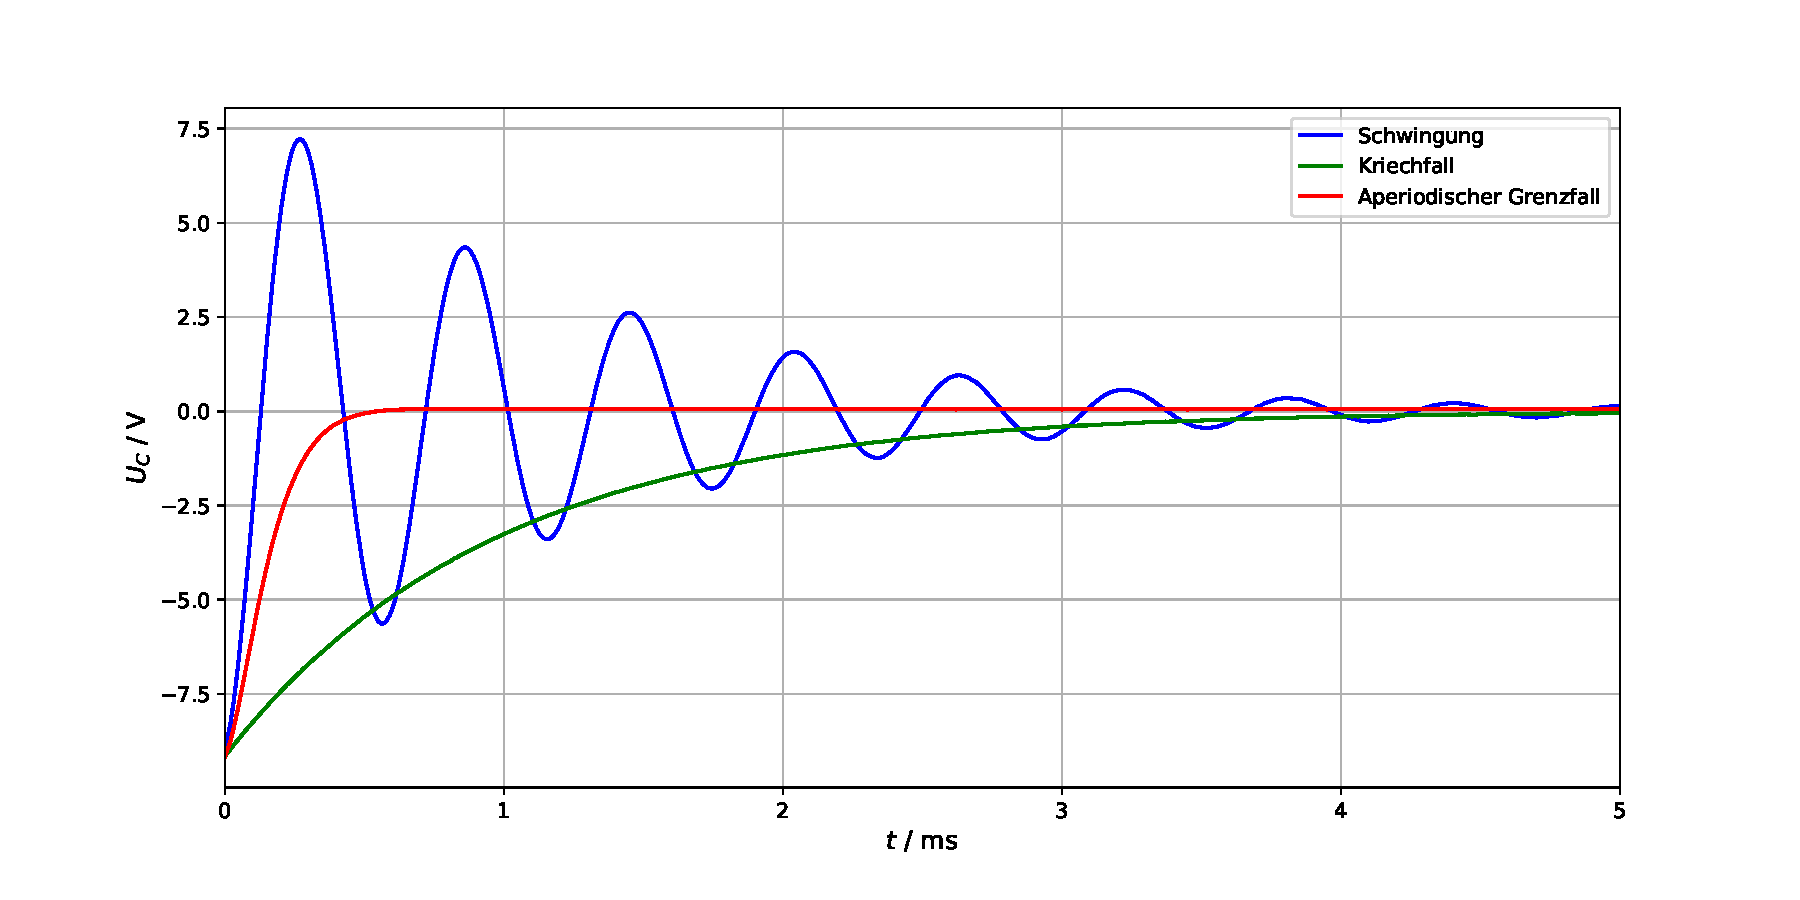
\includegraphics[width=\textwidth]{plots/rohdaten_ska.pdf}
\caption{Rohdaten mit Schwing-, Kriech- und Aperiodischem Grenzfall}
\label{abb:rohdaten_ska}
\end{figure}

\subsubsection{Schwingfall}
Zunächst bestimmen wir die Frequenzen und die Dämpfungen der aufgenommenen Schwingungen für die verschiedenen verwendeten Ohmschen Widerstände. Im folgenden sind die verwendeten Widerstände mit Herstellerangabe und gemessenen Werten angegeben:

\begin{table}[H]
\centering
\begin{tabular}{c|c}
Herstellerangabe / $\Omega$ & Gemessener Wert / $\Omega$ \\
\hline
$1$ & $1.008 \pm 0.001$ \\
$5.1$ & $5.101 \pm 0.001$ \\
$10$ & $9.990 \pm 0.002$ \\
$20$ & $19.82 \pm 0.01$ \\
$47$ & $46.67 \pm 0.01$ \\
$100$ & $99.24 \pm 0.04$ 
\end{tabular}
\end{table}
Für alle nun folgenden Rechnungen wurden die gemessenen Widerstandswerte verwendet. Es existieren zwei Möglichkeiten, um die Frequenz bzw. die Periodendauer zu bestimmen. Einerseits ist die Analyse mittels FFT möglich. Andererseits können die Extrema aus den Rohdaten abgelesen und die Periodendauer mittels Regression über die Schwingungsanzahl bestimmt werden.
Analog dazu besteht die Möglichkeit, die Dämpfung $\delta$ aus Gleichung \ref{eq:i_lsg} durch logarithmisches Auftragen der Extrema, d.h. mit Regression, zu bestimmen: Für die Zeitpunkte $t_i$ an denen $I$ bzw. $U_C$ ein Extremum annimmt, gilt
$$sin(\omega t_i) = \pm 1$$.
Durch logarithmieren der Gleichung erhält man 
$$\log \lvert I(t_i)\rvert = -\delta t_i + \log\left\lvert CU_0 \left(\omega+\frac{\delta^2}{\omega}\right)\right\rvert$$
beziehungsweise eine analoge Form für $U_C$. Natürlich kann $\delta$ durch die Verwendung eines Steigungsdreiecks auch nur bei zwei ablesbaren Maxima oder Minima bestimmt werden:
$$\delta = \frac{\log\left(\frac{U_C(t_0)}{U_C(t_1)}\right)}{t_1-t_0}$$
Bei beiden Vorgehensweisen muss der Offset korrigiert werden.
Eine Regression ist für den $100\Omega$ Widerstand nicht praktikabel, da aufgrund der starken Dämpfung zu wenige Extrema genau ablesbar sind. Ein beispielhaftes Ergebnis für die Regression von abgelesenen Extrema bei der Schwingung des $10\Omega$ Widerstand ist in Abbildung \ref{abb:reg1} dargestellt. Die übrigen durchgeführten Regressionen sind im Anhang \ref{app:reg} abgebildet.

\begin{figure}[h]
\centering
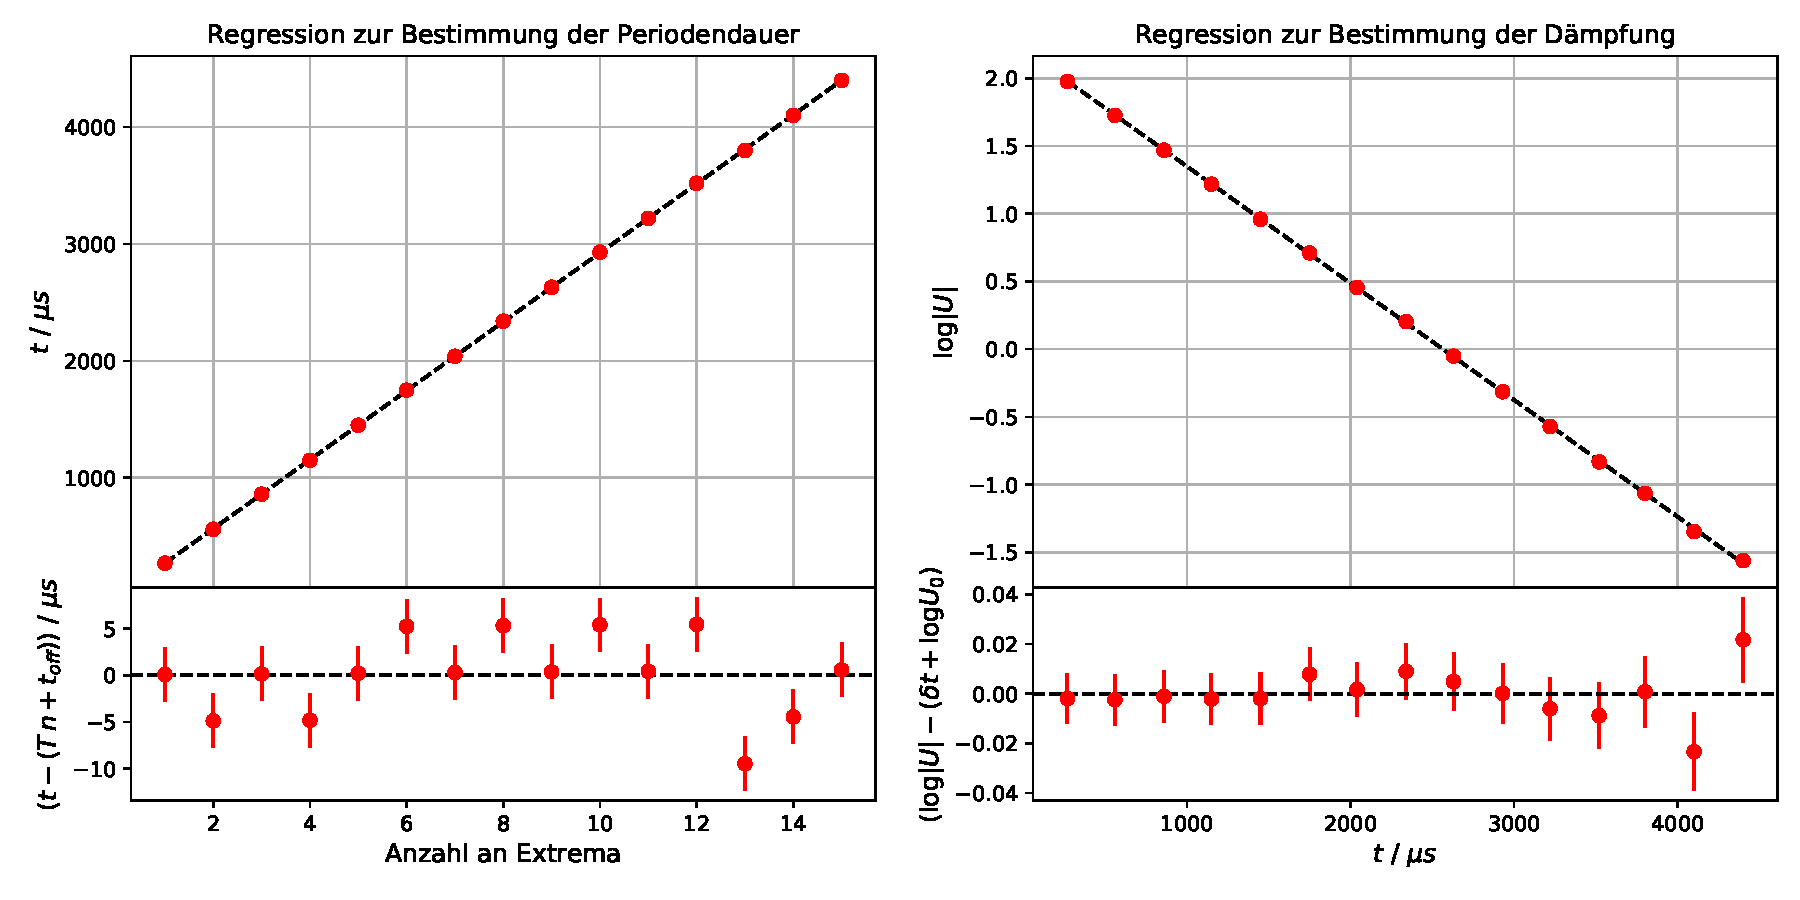
\includegraphics[width=\textwidth]{plots/reg_schwingung3.pdf}
\caption{Regression für den $10\Omega$ Widerstand}
\label{abb:reg1}
\end{figure}

Für die Frequenzen ergeben sich folgende Werte:

\begin{table}[H]
\centering
\begin{tabular}{c|cc}
Ohmscher Widerstand / $\Omega$ & Regression / Hz & FFT / Hz \\
\hline
$1$ & $3393.9 \pm 1.2$ & \\
$5.1$ & $3392.7 \pm 1.4$ & \\
$10$ & $3390.2 \pm 2.0$ & \\
$20$ & $3378.4 \pm 4.3$ & \\
$47$ & $3257.3 \pm 9.7$ & \\
$100$ & - &
\end{tabular}
\end{table}

Folgende Dämpfungswerte wurden berechnet:

\begin{table}[H]
\centering
\begin{tabular}{c|c}
Herstellerangabe / $\Omega$ & Dämpfung / Hz \\
\hline
$1$ & \\
$5.1$ & \\
$10$ &  \\
$20$ & \\
$47$ & \\
$100$ & 
\end{tabular}
\end{table}


\subsection{Fazit}




\section{Gekoppelte LC-Schwingkreise}


\subsection{Versuchsbeschreibung}

In diesem Versuch werden zwei Schwingkreise induktiv miteinander gekoppelt. Speziell werden hier die beiden Fundamentalschwingungen bei gleichsinniger und gegensinniger Anregung und eine Schwebung aufgezeichnet.

\begin{figure}[H]
\centering
\begin{tikzpicture}
% Linke Schwingkreise
\draw (0,0.2) -- (-1,0.2) to [rmeterwa, t=$U_1$] (-1,1.8) -- (0,1.8);
\draw (0.8,0) node[ocirc]{} -- (0,0) to [C, a=$C$] (0,2) -- (2,2) to [cute inductor, a=$L$] (2,0) -- (1.2,0) node[ocirc]{};
\draw (3.55,0) node[ocirc]{} -- (2.75,0) to [cute inductor, a=$L$] (2.75,2) -- (4.75,2) to[C, a=$C$] (4.75,0) -- (3.95,0) node[ocirc]{};
\draw (4.75,0.2) -- (5.75,0.2) to [rmeterwa, t=$U_2$] (5.75,1.8) -- (4.75,1.8);
\draw (2,0) to [normal open switch] (2,-1) -- (0,-1) -- (0,0);
\draw (2.75,0) to [normal open switch] (2.75,-1) -- (4.75,-1) -- (4.75,0);
\draw[dashed, thin] (2.15,-0.5) -- (2.85,-0.5); 


% Rechte Schwingkreise
\draw (8,0.2) -- (7,0.2) to [rmeterwa, t=$U_1$] (7,1.8) -- (8,1.8);
\draw (8.8,0) node[ocirc]{} -- (8,0) to [C, a=$C$] (8,2) -- (10,2) to [cute inductor, a=$L$] (10,0) -- (9.2,0) node[ocirc]{};
\draw (11.55,0) node[ocirc]{} -- (10.75,0) to [cute inductor, a=$L$] (10.75,2) -- (12.75,2) to[C, a=$C$] (12.75,0) -- (11.95,0) node[ocirc]{};
\draw (12.75,0.2) -- (13.75,0.2) to [rmeterwa, t=$U_2$] (13.75,1.8) -- (12.75,1.8);
\draw (10,0) to [normal open switch] (10,-1) -- (8,-1) -- (8,0);
\draw (10.75,0) to [normal open switch] (10.75,-1) -- (12.75,-1) -- (12.75,0);
\draw[dashed, thin] (10.15,-0.5) -- (10.85,-0.5); 

\end{tikzpicture}
\caption{Fundamentalschwingungen der gekoppelten Schwingkreise bei gleichsinniger (links) und gegensinniger Anregung (rechts)}
\end{figure}

Bei überbrückter Spannungsquelle gelten für den gekoppelten Schwingkreis die folgenden Differentialgleichungen 
\begin{align*}
\ddot I_1 + k \ddot I_2 + \frac{1}{LC}I_1 &= 0 \\
\ddot I_2 + k \ddot I_1 + \frac{1}{LC}I_2 &= 0
\end{align*}
Dabei bezeichnet $k \in (0,1)$ die Kopplung der beiden Schwingkreise. 
Mit den sogenannten \textit{Fundamentalströmen} $I_+ = I_1 + I_2$ und $I_- = I_1 - I_2$ erhält man durch Addition bzw. Subtraktion der obigen Gleichungen und anschließendem Umformen
\begin{align*}
\ddot I_+ + \frac{1}{LC(1+k)} I_+ = 0 \\
\ddot I_- + \frac{1}{LC(1-k)} I_- = 0
\end{align*}
Daraus ergeben sich harmonische Schwingungen mit den Kreisfrequenzen 
$$\omega_+ = \frac{\omega_0}{\sqrt{1+k}} \hspace{0.2cm} \text{ und } \hspace{0.2cm} \omega_- = \frac{\omega_0}{\sqrt{1+k}}.$$
Dabei ist $\omega_0 = \frac{1}{\sqrt{LC}}$ die Kreisfrequenz der ungekoppelten Schwingung. Mithilfe der Fundamentalschwingungen lässt sich dann der Kopplungsgrad bestimmen
$$k = \frac{f_-^2 - f_+^2}{f_-^2 + f_+^2}.$$
Bei Messung einer Schwebung mit Schwebungsfrequenz $f_s$ und Frequenz der gekoppelten Schwingung $f_k$ kann man die Fundamentalschwingungen gemäß
$$f_k = \frac{f_- + f_+}{2} \hspace{0.2cm} \text{ und } \hspace{0.2cm} f_s = \frac{f_- - f_+}{2}$$
bestimmen. Aufgrund der unvermeidbaren Dämpfung der beiden Schwingkreise sind die Extrema des einen Schwingkreises gegen die Nulldurchgänge des anderen verschoben. Für Kopplungen $k < 0.2$ gilt näherungsweise für die zeitliche Verschiebung
$$\Delta t \approx \frac{1}{\omega_s} \left( \frac{\pi}{2} - \arctan\left(  \frac kR \sqrt{\frac LC}\right) \right).$$


\subsection{Versuchsaufbau}

\subsection{Versuchsdurchführung}

\subsection{Versuchsauswertung}

\subsection{Fazit}

\appendix
\section{Regressionen der übrigen Widerstände}\label{app:reg}
\begin{figure}[h]
\centering
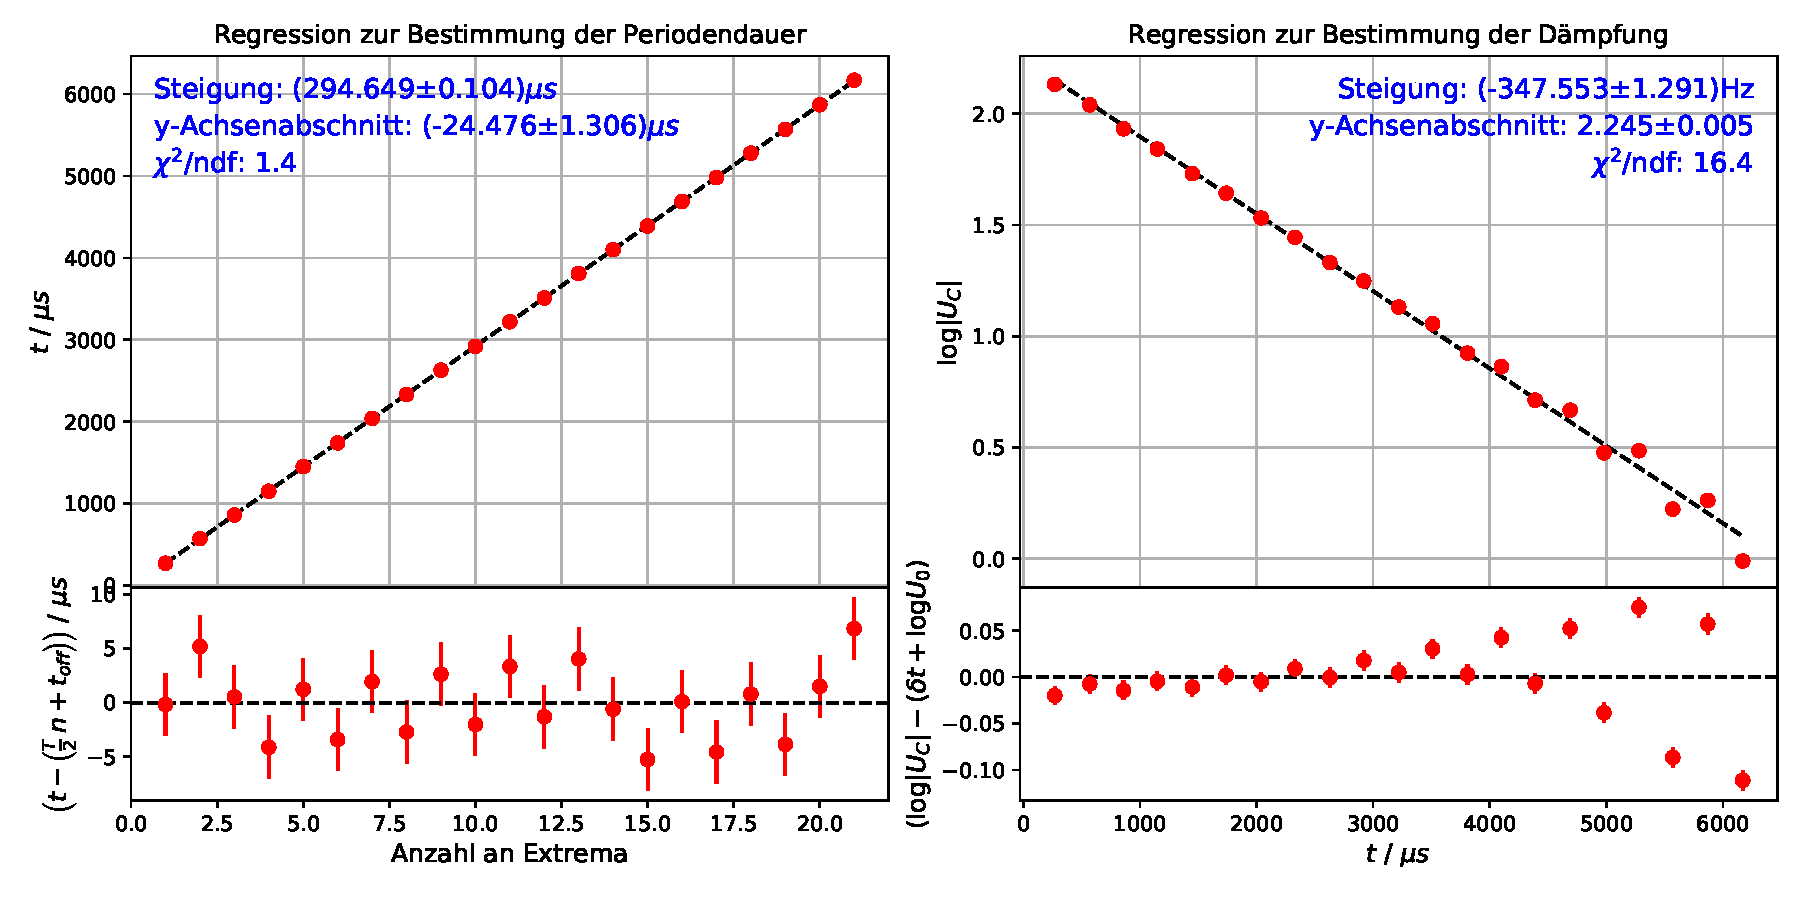
\includegraphics[width=\textwidth]{plots/reg_schwingung1.pdf}
\caption{Regression für den $1\Omega$ Widerstand}
\end{figure}
\begin{figure}[h]
\centering
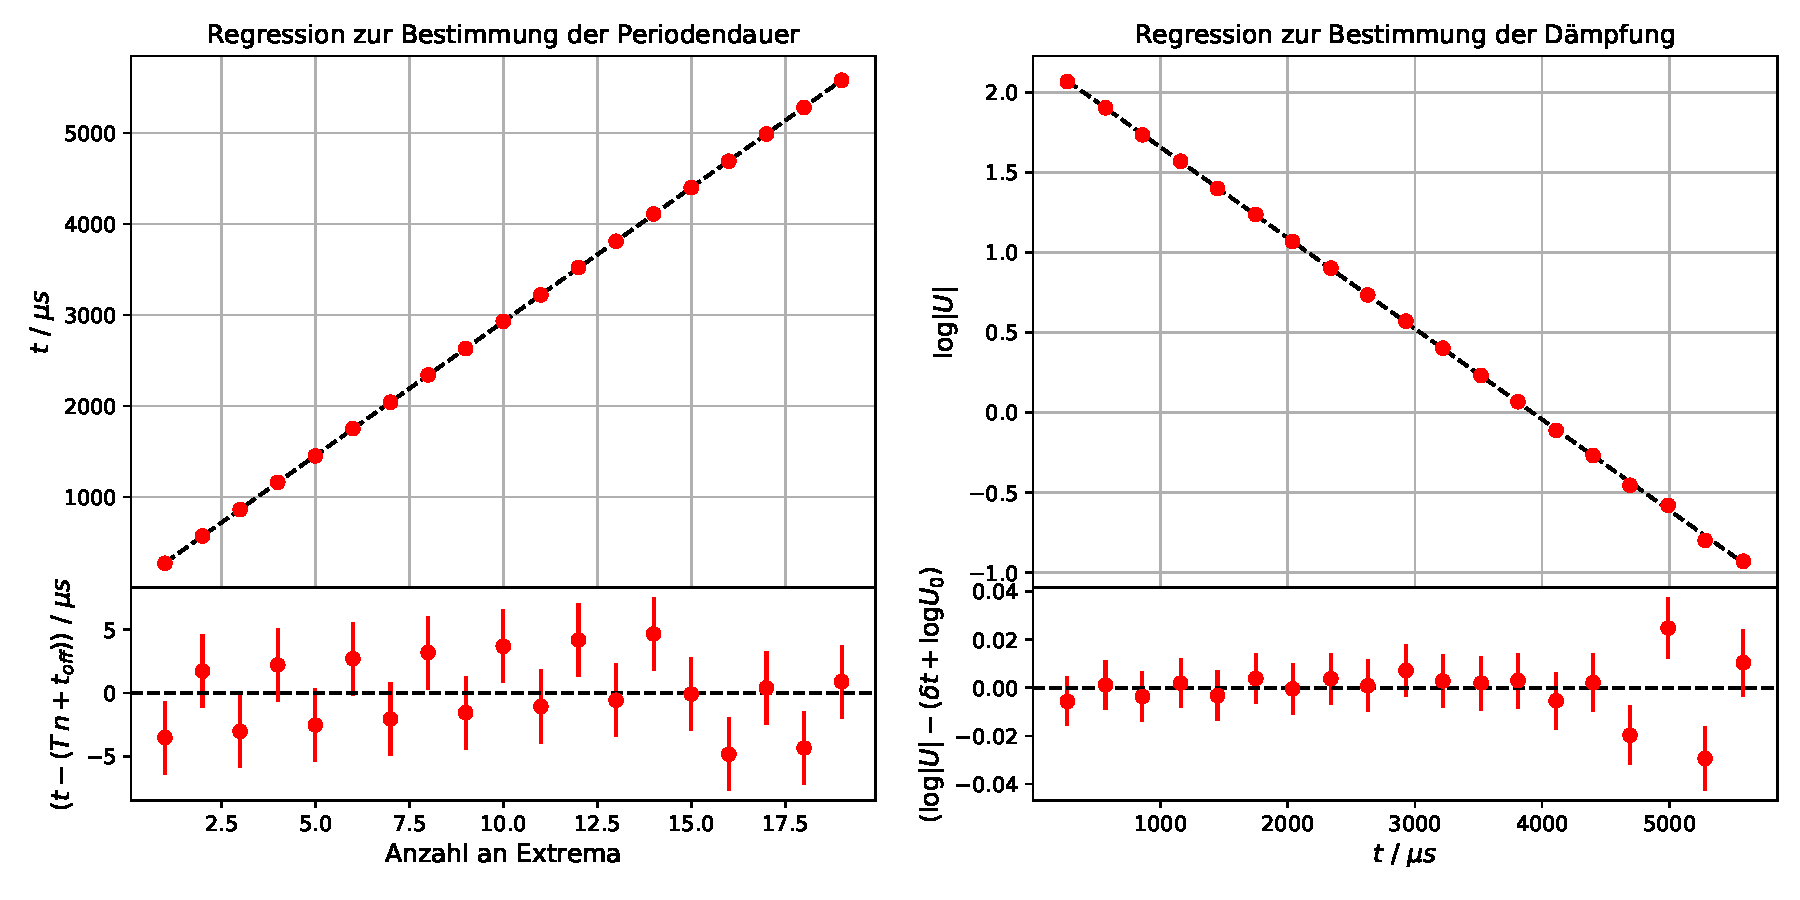
\includegraphics[width=\textwidth]{plots/reg_schwingung2.pdf}
\caption{Regression für den $5.1\Omega$ Widerstand}
\end{figure}
\begin{figure}[h]
\centering
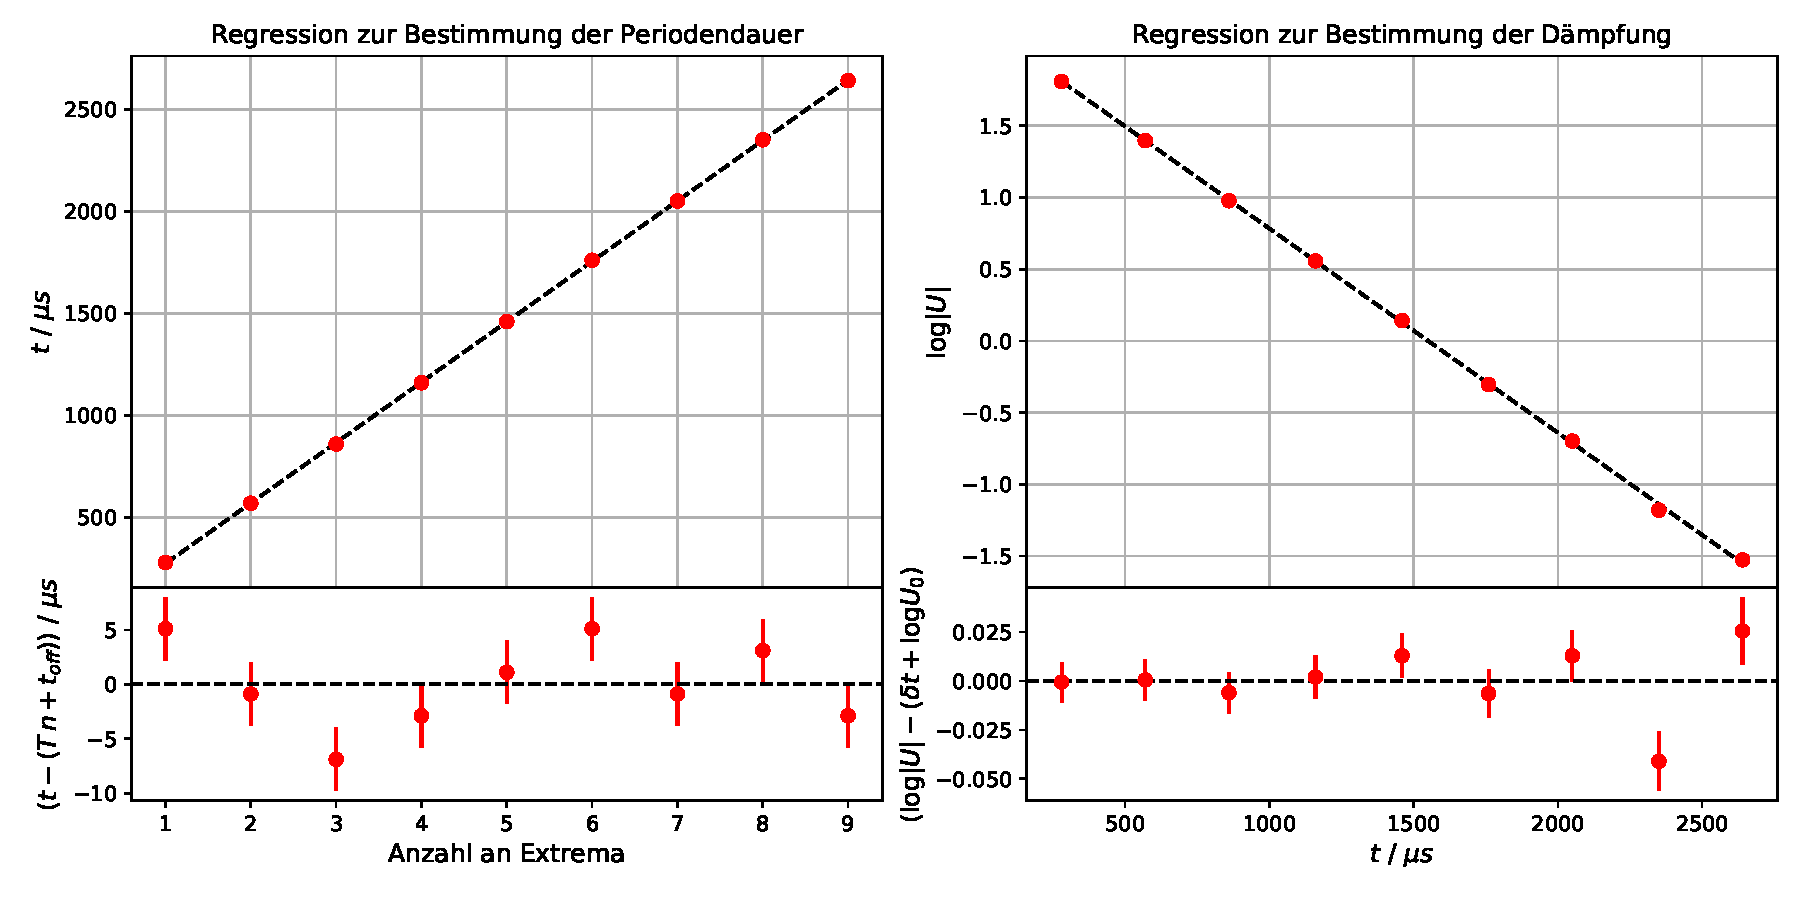
\includegraphics[width=\textwidth]{plots/reg_schwingung4.pdf}
\caption{Regression für den $20\Omega$ Widerstand}
\label{abb:reg1}
\end{figure}
\end{document}